\section{Administration}
This section describes the administrative functionality. 
It covers usage history, route history, booking routes, and an add/remove page.
It also contains a bicycle GPS tracking, but this has been mentioned in \secref{sec:googlemapsapi}.

\subsection{Route History}
This part of the administration site handles showing a map of the historical locations of a bicycle.
The admin provides one or more bicycles, a start, and end date.
Then if there are historical GPS coordinates for the bicycle(s), they will be shown on the map. 

The purpose of the route history page is to give the admins an idea of which roads the bicycles are traveling a lot on. 
This can then be used as a decision-making tool to decide where to put new stations, in that if the admin can see that a lot of bicycles are traveling to a specific point it might be a good idea to put a station there.
It could also be used to see if a specific bicycle is being 'misused' in the sense that it would be visible if the bicycle is only being used to travel to one spot and nowhere else.

See \figref{fig:routehistory} for a figure of what the page looks like.

\begin{figure}[H]
	\centering
	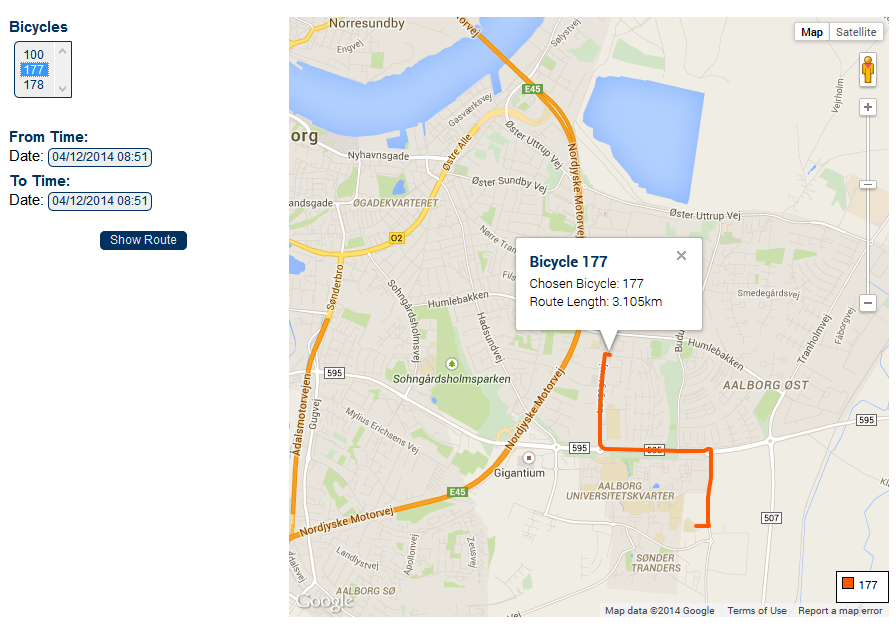
\includegraphics[scale=0.75]{RouteHistory.png}
	\caption{Picture of Route History}
	\label{fig:routehistory}
\end{figure}


\subsection{Booking Routes}
%This part of the administration site handles showing a map of the routes associated with a booking. Skal det bruges til noget???

\subsection{Add/Remove}
This part of the administration site handles the adding and removing of users, bicycles, docks, and stations.

\begin{description}[style=nextline]
\item[User] 
The admin can add a normal user and set up his or her details or the admin can add another admin.
Removal of users by the admin is also provided functionality.
However, while the admin can remove all other users and admins he cannot remove himself.
\item[Bicycle] 
Functionality for adding bicycles was added, this requires no information about the bicycle being given.
The reason why no dock have to be given when adding a bicycle is because the bicycle has to be inserted manually into a dock.
While addition of bicycles require no information being provided, removal of bicycles requires providing the id of the bicycle.
Furthermore, the admin should remove the bicycle from the dock it is located at, before it is removed from the system.
\item[Dock] 
Addition of docks requires the admin choosing which station to which the dock has to be added.
After adding a dock, the station has to be notified because the database on the station has to be updated.
Removal of docks requires the admin choosing which dock at which station to remove from, with the notice that it only allows removal of docks not currently used.
After removing a dock the station containing the dock has to be notified that the dock have been removed from the station.
\item[Station] 
Adding a station requires information about the name, the coordinates, and the ip address, given that we simulate the stations we also need to notify the station software that a new station has been added, however, this is not needed for the final version as ours only work as a prototype.
Removal of station requires the admin to choose which station that has to be removed.
The admin will be warned that removing this station will also remove all the docks and detach the bicycles from the removed docks.
In our simulated world the station software also needs to be notified to update the database, just as adding a new station this is not needed for the final version.
\end{description}
See \appref{app:addremove} for a picture of the administration page.